\documentclass[conference]{IEEEtran}

\usepackage{mathptmx} % Times Roman Font

\usepackage{helvet} % Arial/Helvetica font
\renewcommand{\familydefault}{\sfdefault} % Makes serif text all Helvetica

\usepackage[left=0.5cm, right=0.5cm, top=0.5cm]{geometry} % Sets the page margins

\usepackage{graphicx}

\usepackage{multicol}
\usepackage{float}

\usepackage{caption}

\captionsetup[table]{skip=10pt} % Adjusts space between table and caption


\usepackage{ragged2e}

\title{Case Study 1: Gait Analysis}
\date{}

\begin{document}
\justifying

\maketitle

\section{Introduction} % The start of a new section
This report compares the differences of gait in two controls, and two subjects with Spina Bifida. Spina Bifida is a birth defect that affects a person's mobility - ranging from mild to severe. Gait analysis is the study of motion. Differences in people's gait cycles can help us identify problems they may be facing. The position data was collected using a markerless system.

\section{Methods}\label{methods}

The position data was collected using a markerless system \cite{geerse2015kinematic}. Markers analysed in this report include: walking speed, stride length, ankle dorsiflexion, knee angle, lumbar bending, hip flexion. (STRN, LHEE, RHEE, LANK, RANK).

\subsection{Walking Speed and Stride Length}

Walking speed was measured by calculating the forward (X-axis) displacement of the STRN (sternum) marker and dividing it by the duration of the gait study.

Stride length was calculated by measuring the horizontal displacement of the heel marker between consecutive heel strikes during gait cycles. Heel strikes were identified using velocity thresholds and positional criteria. For each stride, the distance travelled by the heel marker from one heel strike to the next was calculated to obtain stride length. The average stride length for each patient was then computed.

\subsection{Joint Angles}

Knee flexion and extension was plotted against the gait cycle to assess mobility during the stance and swing phases. Comparing these angles allows for identification of reduced range of motion (ROM) or delayed peak flexion.

Thoracic lateral sway was measured from the lumbar bending angle. Increased sway may suggest compensatory movement due to lower limb weakness or balance issues.

Ankle dorsiflexion was measured from the leading leg's ankle angle. The angles were analysed during the toe-off stage of the gait cycle to evaluate dorsiflexion capability.

\section{Results}\label{results}

\subsection{Gait Waveforms}

Comparing the knee angle of the leading leg over time of all four individuals, in Figure.~\ref{fig:Gaitcollage}, both controls exhibit typical gait characteristics with stanceand swing phases lasting approximately 55\% and 45\% of the gait cycle, respectively.

In contrast, subject 1 shows a large decrease in swing phase duration (approximately 25\%) and a maximum knee flexion of 35°. These decreases suggest that the subject may have difficulty initiating or completing a leg swing.

Subject 2 shows a more typical gait pattern with a swing phase of approximately 40\% and maximum knee flexion of 63°, which closely matches the controls. This indicates that the subject may have a milder form of Spina Bifida.

Both subjects have multiple knee flexion peaks during the stance phase. These are not present in the controls. These represent instability or movements to compensate for problems with balance.


\begin{figure}[h]
\centering
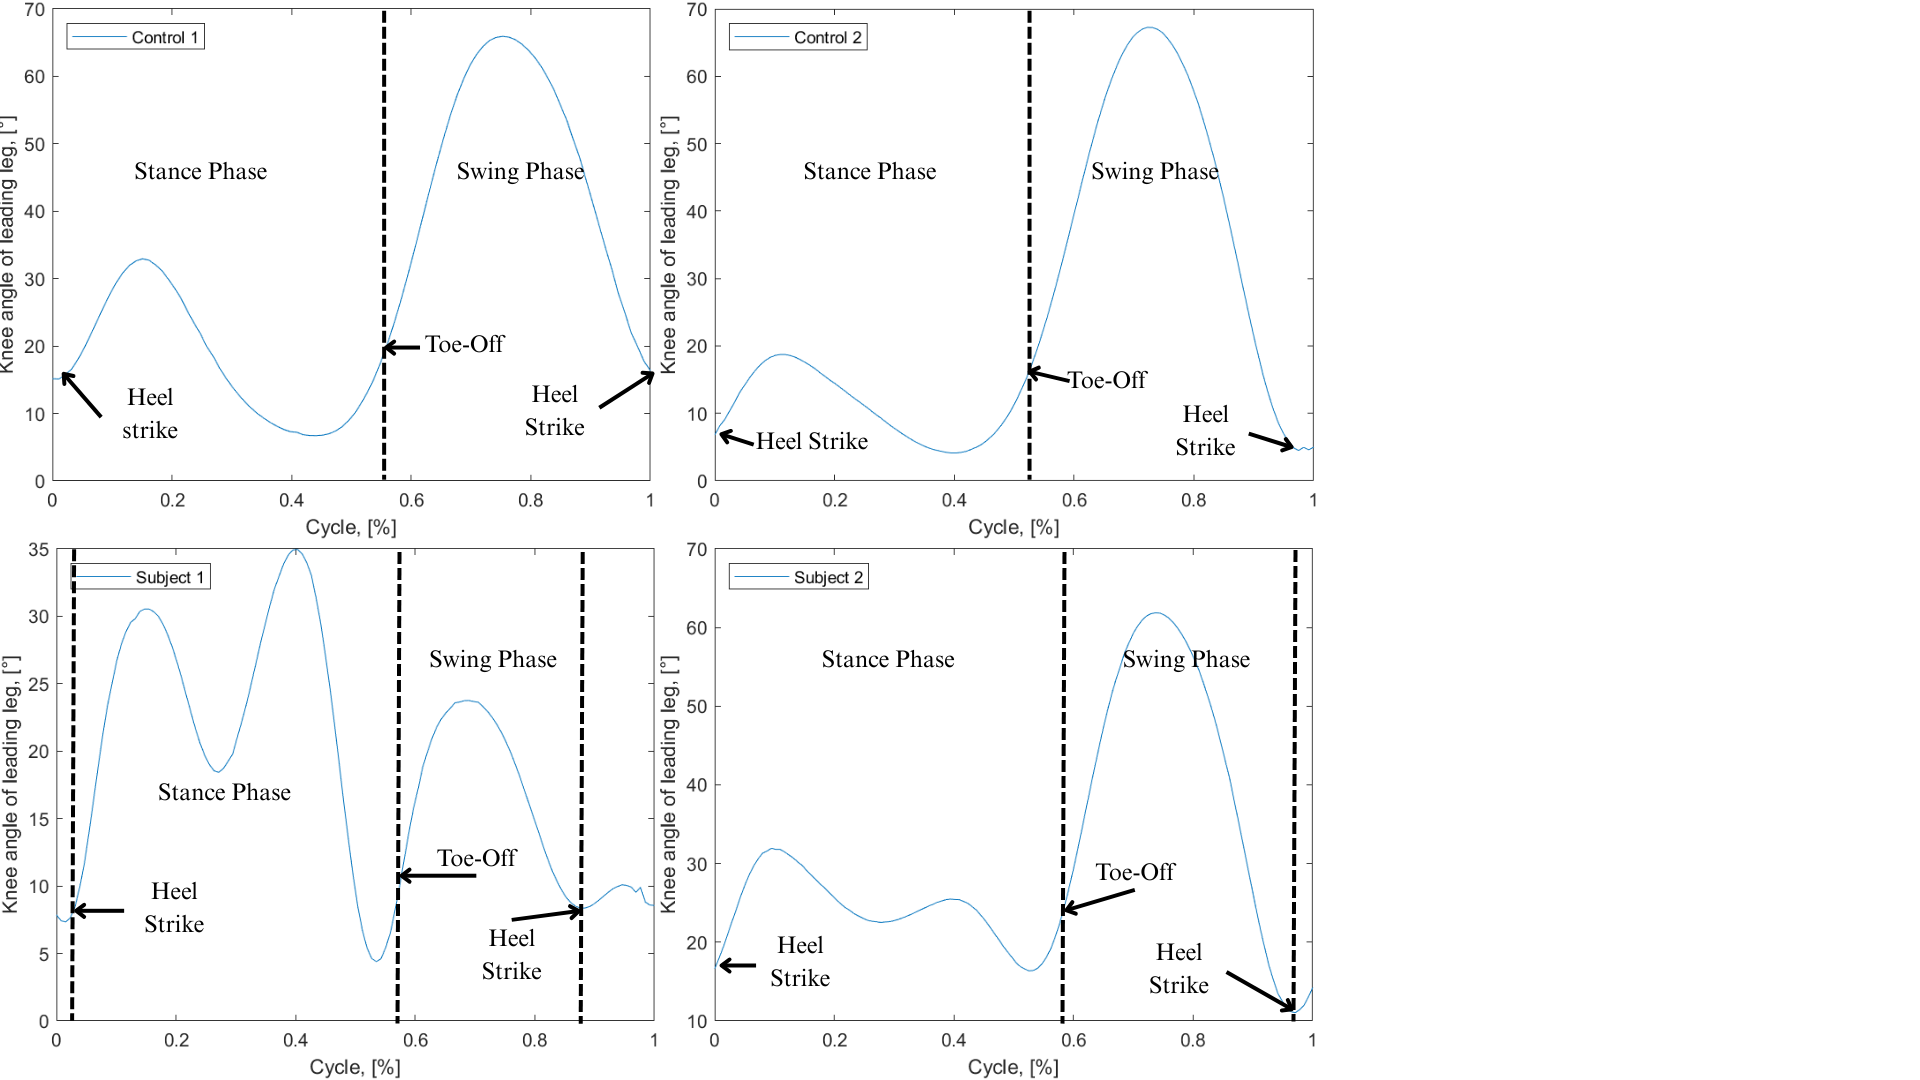
\includegraphics[width=14cm]{Gait cycle collage.png}
\caption{The labelled gait cycle for the leading left knee of each of the participants}
\label{fig:Gaitcollage} % this gives the figure a unique name that you can refer to in the main text \ref{fig:...}
\end{figure}

\subsection{Walking Speed and Stride Length}

From Table.~\ref{tab:speedStrideData}, control 1 has the largest average walking speed, followed by control 2. In contrast, both subjects have a reduced average walking speed. Subject 2 has the lowest average speed, over 30\% slower than control 1.

The average stride length is also reduced in both subjects. The controls had an average stride length of 1.09m while the subjects had an average stride length of 0.77m. Subject 2 had the largest reduction in stride length, 29\% slower than control 1.

These results are consistent with mobility issues as a result of Spina Bifida, with reduced lower limb strength, joint control, and balance. 

\begin{table}[h]
\centering
\begin{tabular}{|c|c|c|}
\hline
Participant & Walking Speed (m/s) & Average Stride Length (m) \\
\hline
Control 1 & 1.476 & 1.190 \\
Control 2 & 1.172 & 0.998 \\
Subject 1 & 1.146 & 0.938 \\
Subject 2 & 1.021 & 0.610 \\
\hline
\end{tabular}
\caption{Results from walking speed and stride length calculations}
\label{tab:speedStrideData}
\end{table}


\subsection{Ankle Dorsiflexion}

\begin{figure}[!ht]
\centering
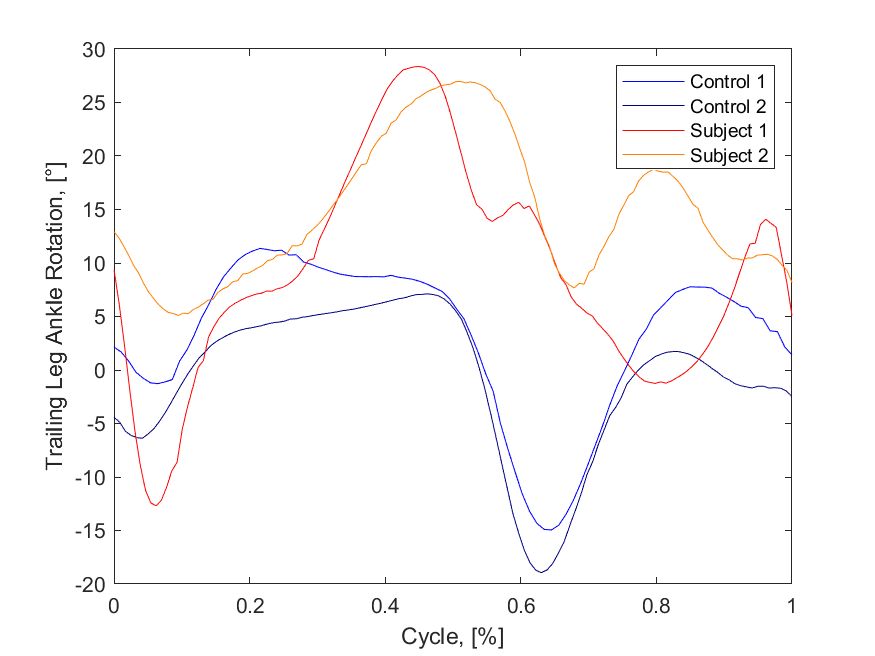
\includegraphics[width=10cm]{leading leg ankle rotation.png}
\caption{Dorsiflexion of the leading leg ankle over a single gait cycle}
\label{fig:LeadingAnkleDorsiflexion}
\end{figure}

Figure.~\ref{fig:LeadingAnkleDorsiflexion} shows the ROM of the leading leg's ankles. Both subjects show reduced plantarflexion across the gait cycle. This suggests that the subjects have decreased propulsion at toe-off.

Also, both subjects show an increased dorsiflexion preceding toe-off. The subjects show an increased ROM in ankle angles 10° greater than the control group. This could represent compensatory movements due to reduced muscle strength or limited ankle plantarflexion control.

\subsection{Hip Flexion}

\begin{figure}[!ht]
\centering
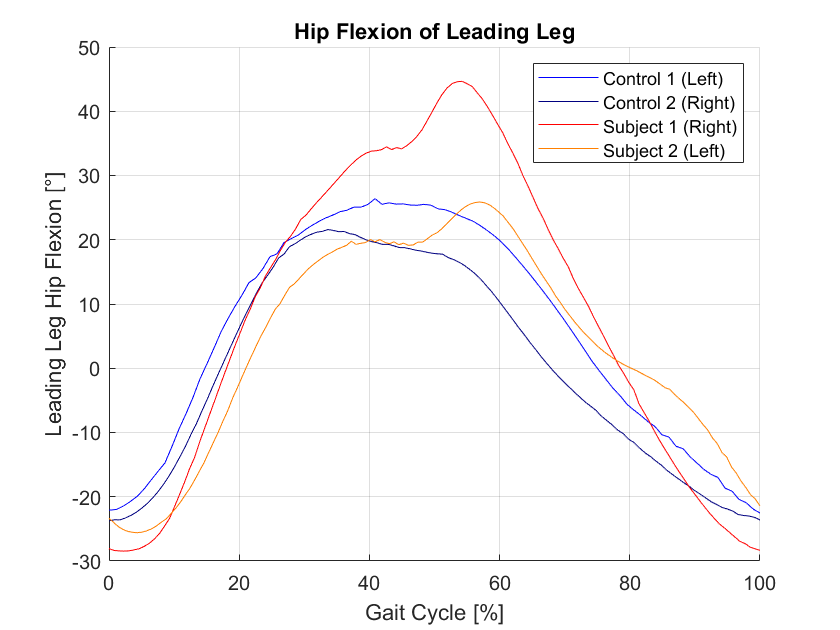
\includegraphics[width=10cm]{hipflexion.png}
\caption{Hip flexion over the period of a single gait cycle}
\label{fig:HipFlexion}
\end{figure}

Figure.~\ref{fig:HipFlexion} shows the hip flexion angles throughout the gait cycle. The controls show a typical hip flexion ROM of 45-50°.

However, the subjects show an increased ROM of 50-70°. Also, both subjects show clear peaks in hip flexion preceding toe-off. These are not seen on the controls. These are likely a result of compensatory motions to assist with balance or muscle weakness.

\subsection{Lumbar}

\begin{figure}[!ht]
\centering
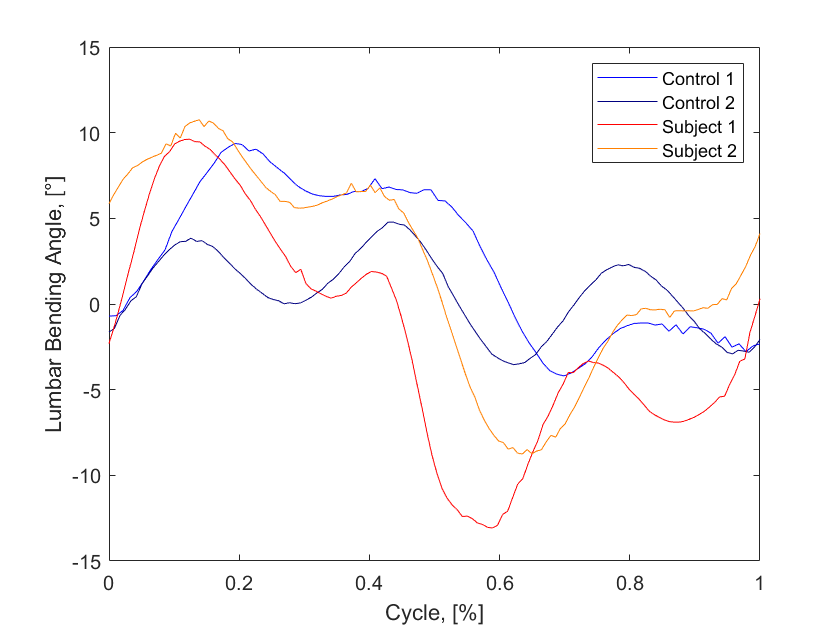
\includegraphics[width=10cm]{LumbarBending.png}
\caption{Lumbar bending over the period of a single gait cycle}
\label{fig:LumbarBending}
\end{figure}

Figure.~\ref{fig:LumbarBending} shows the thoracic lateral sway over the gait cycle. Subject 1 and 2 have a maximum lumbar ROM of 13° and 9°, respectively. This is increased from the controls ROM of approximately 4°. Both maxima are achieved preceding toe-off.

The increased ROM is likely a result of compensatory motions to assist with balance or muscle weakness.

\subsection{Limitations of Data}

The small sample size limits the ability to draw statistically significant conclusions.

Also, the variation in participant characteristics may have introduced confounding variables. Height and weight can greatly effect gait, making direct comparisons less reliable.

Furthermore, a markerless system is less accurate than marker based systems. Errors in measurements can propagate through inverse kinematic calculations, effecting angle measurements.

\section{Conclusions}\label{conclusions}

To conclude, both subjects show clear signs of Spina Bifida compared to the controls. Both subjects have decreased walking speed, stride length, Knee ROM, increased ankle dorsiflexion, and increased lumbar and hip ROM. These suggest that the subjects are using compensatory motions to assist with balance or muscle weakness.

The sample size reduces the precision of results. Future studies should include more participants and implement a marker based system.



\bibliographystyle{IEEEtran}
% \bibliography{references} 
\end{document}